\documentclass[a4paper,10pt]{article}
\usepackage[utf8]{inputenc}
\usepackage{graphicx}
\usepackage{hyperref}
\usepackage{verbatim}
\usepackage[section]{placeins}

\graphicspath{
    {img/}
}

%opening
\title{}
\author{Jan Toušek}
\author{Ladislav Prix}

\author{
  Toušek, Jan\\
  \texttt{touseja4@fit.cvut.cz}
  \and
  Prix, Ladislav\\
  \texttt{prixladi@fit.cvut.cz}
}

\begin{document}

\begin{titlepage}
   \begin{center}
       \vspace*{0.5cm}
       
\includegraphics[width=0.6\textwidth]{logo_FIT.pdf}
       
       \vspace{2cm}
       \textbf{R-strom}
 
       \vspace{0.5cm}
       Projektová dokumentace k implementaci R-stromu
 
        {\let\newpage\relax\maketitle}
       \maketitle

       \vfill
 
       Vypracováno jako semestrální projekt v předmětu BI-VWM\\
 
       \vspace{0.8cm}
 

 
       Katedra softwarového inženýrství\\
       České vysoké učení technické v Praze\\
       Fakulta informačních technologií\\
 
   \end{center}
\end{titlepage}

%\maketitle

\clearpage
\begin{abstract}
Tento dokument obsahuje projektovou dokumentaci k semestrálnímu projektu pro předmět BI-VWM. Jde o implementaci R-stromu a webového grafického rozhraní, které umožňuje provádět nad stromem operace vložení, dotazování a ukládání.
\end{abstract}

\clearpage

\section{Popis projektu}
Cílem této práce bylo vytvořit vlastní implementaci R-Stromu. R-strom je hyerarchická datová struktura, založena na B+-stromu. Je používán pro indexaci d-dimenzionálních objektů, které jsou reprezentovány jejich minimálním ohraničujícím obdélníkem - Minimum Bounding Rectangle, dále MBR. \cite{rtree}

\subsection*{Vstupy}
Vstupy jsou tvořeny náhodně vygenerovanými daty, nebo daty zadanými uži-vatelem. Nicméně díky vytvořenému API je možné snadno importovat do stromu jakákoliv data, pokud se jedná o body v d-dimenzionálním prostoru.

\subsection*{Výstupy}
Výstupem jsou pak výsledky vyhledávání pomocí různých typů dotazů (Range query, Nearest neighbour query\dots). 
\section{Způsob řešení}
Objekty, se kterými strom pracuje jsou body v n-dimenzionálním prostoru. Tyto body jsou uloženy v listech stromu. Každý uzel stromu je definován svým MBR, který obsahuje všechny uzly - pokud je uzel vnitřní, nebo body - pokud jde o list.

\subsection{Implementované metody}
Pro R-Strom jsme naimplementovali následující metody


\subsubsection*{Insert}
Umožňuje vložit nový bod do stromu. Použili jsme algoritmus Insert, popsaný v knize R-trees: theory and applications.\cite{rtree} Tento algoritmus jsme upravili pro naši potřebu, protože pracujeme s body. Při vkládání nového bodu do stromu záleží na použtém algoritmu dělení uzlů, pokud se některý uzel zaplní. Naimplementovali jsme tři různé algoritmy - lineární, kvadratický a exponenciální. Porovnání těchto algoritmů a jejich výhody a nevýhody jsou blíže popsány v sekci \ref{sec:exp}.

\subsubsection*{Contains}
Vrátí, jestli strom obsahuje zadaný bod.


\subsubsection*{RangeQuery}
Pro zadaný bod a rozsah vrátí všechny body, které se necházejí v daném rozsahu.


\subsubsection*{NNQuery}
Nearest Neighbour query. Vrátí bod, který se nachází nejblíže zadanému bodu.


\subsubsection*{KNNQuery}
Vrátí $k$ nejbližších bodů zadanému bodu.


\section{Implementace}
\subsection{Architektura}
Rozhodli jsme se vytvořit pro R-strom uživatelské rozhraní v podobě webové aplikace. Toto rozhraní komunikuje s API, které na serveru pracuje s daným R-stromem. Obrázek \ref{fig:architektura}
\begin{figure}
    \centering
    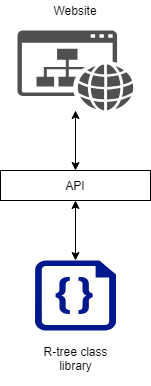
\includegraphics[width=.3\textwidth]{Diagram.png}
    \caption{Architektura projektu}
    \label{fig:architektura}
\end{figure}


\subsection{Zvolené technologie}
Backend a API jsme napsali v jazyku C\# s využitím frameworku .NET Core. Webová aplikace je vytvořena v JavaScriptu. Pro tyto technologie jsme se rozhodli, protože s nimy máme dobré zkušenosti a protože nám poskytly veške-rou potřebnou funkcionalitu. Jako vývojové prostředí jsme použili Visual Studio 2017 Community a Visual Studio Code.

\subsection{Použité knihovny}
\subsubsection*{Backend}
\begin{description}
	\item[Newtonsoft.Json] -- výkonný JSON framework pro .NET\cite{newtonsoft}
    \item[NETStandard.Library] -- meta knihovna pro .NET core projekty\cite{netstandard}
\end{description}

\subsubsection*{API}
\begin{description}
	\item[Microsoft.AspNetCore.All] -- defaultní API pro ASP.NET Core aplikace\cite{aspnetcore}
    \item[Microsoft.NETCore.App] -- defaultní API pro .NET Core aplikace\cite{netcore}
    \item[Microsoft.Extensions.PlatformAbstractions] -- abstrakce pro .NET Framework, .NET Core a Mono API\cite{abstractions}
    \item[Swashbuckle.AspNetCore] -- nástroj Swagger pro tvorbu dokumentace API, vytvořených v ASP.NET Core \cite{swagger}
\end{description}

\subsubsection*{Frontend}
\begin{description}
	\item[React] -- JavaScript knihovna pro tvorbu uživatelských rozhraní\cite{react}
    \item[Ant Design] -- knihovna pro grafický design webových aplikací\cite{ant}
    \item[Konva] -- knihovna pro kreslení ve 2d\cite{konva}
\end{description}


\subsection{Požadavky pro spuštění}
Aby bylo možné projekt spustit, je potřeba mít nainstalované následující:

\begin{description}
	\item[.NET Core SDK] -- .NET platforma \cite{dotnet}
    \item[Node.js] -- JavaScript runtime \cite{nodejs}
    \item[Node package manager] -- správce JavaScript balíčků \cite{npm}
\end{description}

\subsection{Spuštění na platformě Windows}
\subsubsection*{Backend}
Pro build backend části je potřeba přesunout se z kořenového adresáře projektu do složky API.

\begin{verbatim}
    cd ./server/Vwm.RTree.Api
\end{verbatim}
A poté spustit powershell script BuildAndRun.ps1, který sestaví a spustí projekt API v konfiguraci Release. API je pak defaultně k dispozici na adrese~\url{http://localhost:8080/} \ref{fig:buildandrun}
\begin{figure}
\label{fig:buildandrun}
\caption{Script BuildAndRun.ps1}
\begin{verbatim}

param(
[switch] $noBuild)

if(!$noBuild)
{
   dotnet build --configuration Release
}
dotnet exec .\bin\Release\netcoreapp2.2\Vwm.RTree.Api.dll
\end{verbatim}
\end{figure}

\subsubsection*{Frontend}
Pro build frontendu se přesunout do složky front a spustit příkazy npm install a npm start. Webová aplikace běží defaultně na adrese \url{http://localhost:3000/}
\begin{verbatim}
    cd ./front
    npm install
    npm start
\end{verbatim}





\section{Příklad výstupu}
Pro zadávání vstupů a zobrazení výstupů jsme vytvořili webovou aplikaci, která umožňuje používat všechny metody implementované na R-stromu. Níže popíšu záložky, které tato aplikace obsahuje a přidám screenshoty s ukázkami vstupů a výstupů.

\subsection{Webová aplikace}
\subsubsection*{Add Point}
Umožňuje přidávat body do R-stromu. Obrázek \ref{fig:addpoint}.
\begin{figure}
    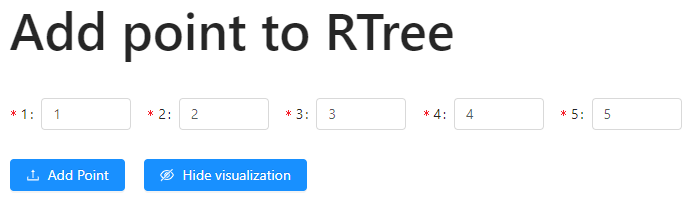
\includegraphics[width=\textwidth]{AddPoint.png}
    \caption{Záložka Add Point}
    \label{fig:addpoint}
\end{figure}
\subsubsection*{Dotazy}
V rozhraní pro dotazy má uživatel dvě možnosti provedení dotazu. 

\begin{description}
	\item[Perform Query] - provede dotaz nad R-stromem, vrátí výsledky a zobrazí dobu trvání dotazu
    \item[Perform query with benchmark] - provede dotaz nad R-stromem i lineárně a zobrazí oba výsledky a čas trvání obou dotazů pro možné porovnání
\end{description}


\subsubsection*{Range Query}
Umožňuje zadat bod a rozsah, ve kterém se mají nacházet výsledky. Vyhledané výsledky vrátí a zobrazí. Obrázek \ref{fig:rangeq}.
\begin{figure}
    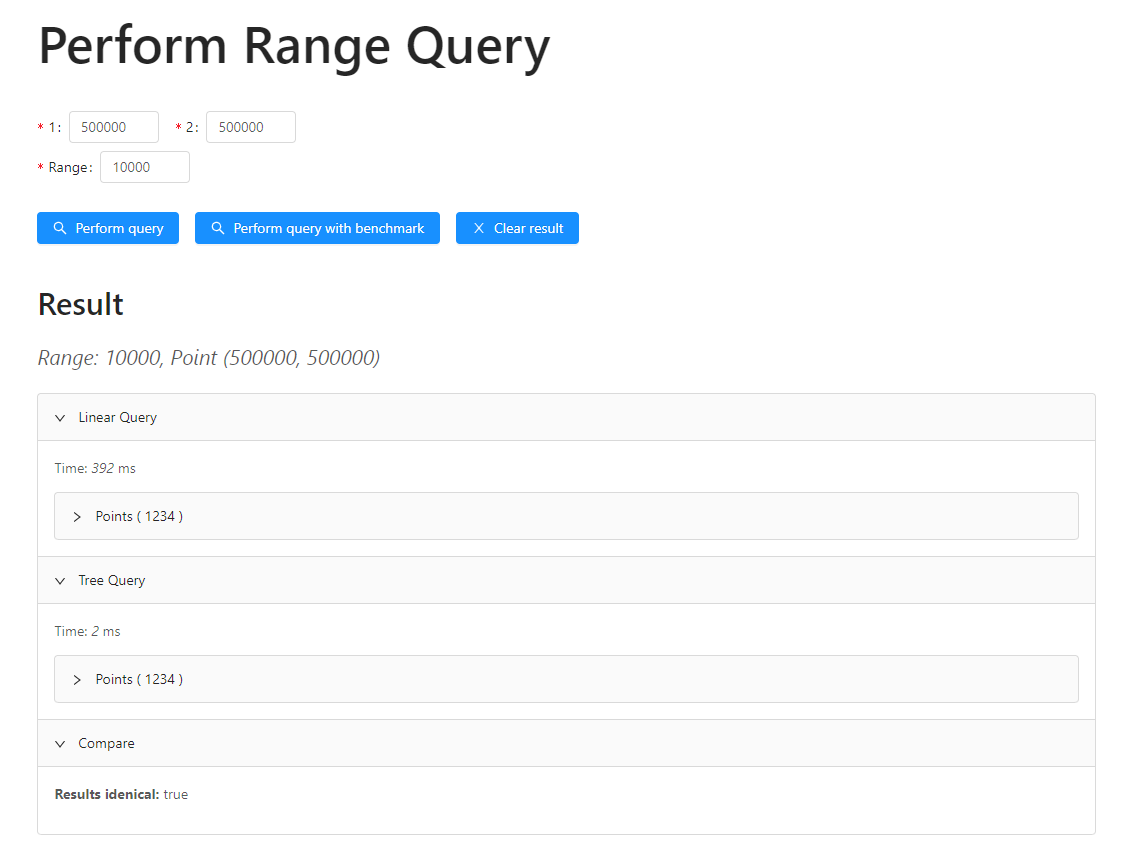
\includegraphics[width=\textwidth]{RangeQuery.png}
    \caption{Záložka Range Query}
    \label{fig:rangeq}
\end{figure}
\subsubsection*{NN Query}
Umožňuje zadat bod a vyhledat bod, který je k němu nejblíže. Obrázek \ref{fig:nnq}.
\begin{figure}
    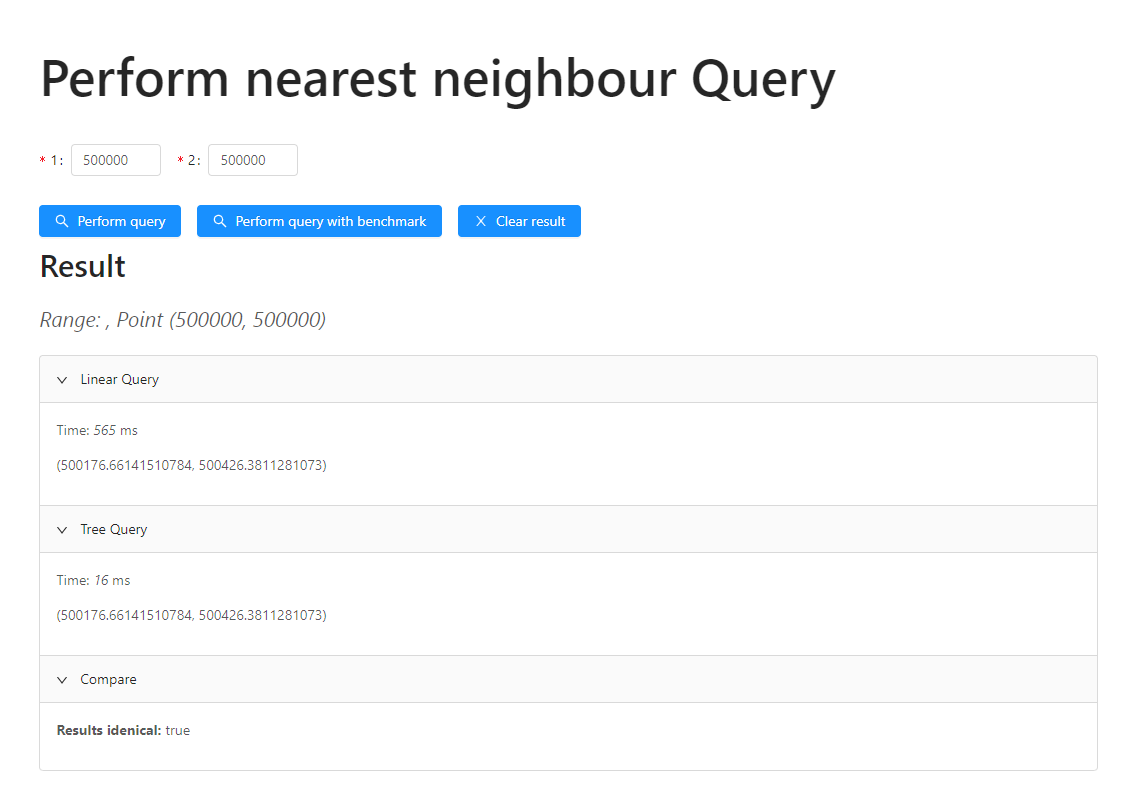
\includegraphics[width=\textwidth]{NNQuery.png}
    \caption{Záložka NN Query}
    \label{fig:nnq}
\end{figure}

\subsubsection*{KNN Query}
Umožňuje zadat bod a vyhledat $k$ bodů, které jsou k němu nejblíže. Obrázek \ref{fig:knnq}.
\begin{figure}
    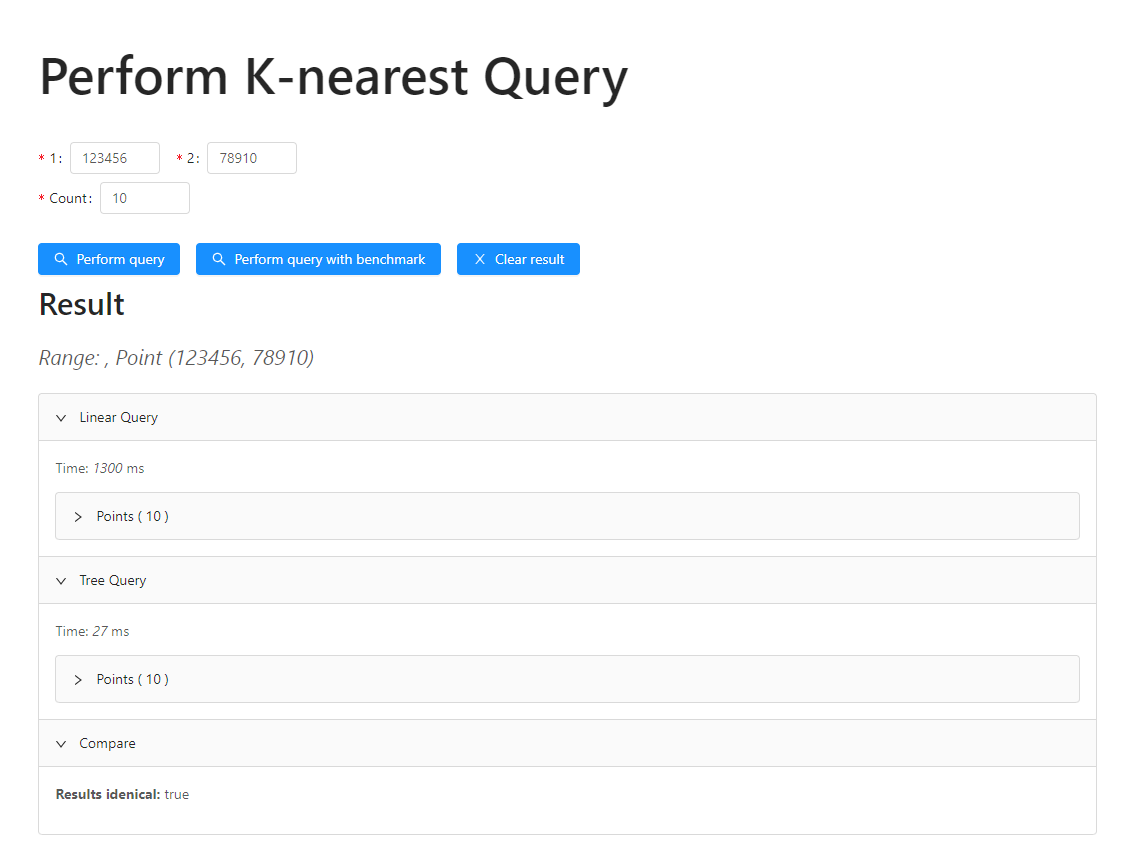
\includegraphics[width=\textwidth]{KNNQuery.png}
    \caption{Záložka KNN Query}
    \label{fig:knnq}
\end{figure}
\subsubsection*{Contains}
Prohledá R-strom a zjistí, jestli obsahuje zadaný bod.

\subsubsection*{Data}
Na záložce data je možné zobrazit strukturu stromu, včetně bodů, které strom obsahuje. Obrázek \ref{fig:data}. Dále zde najdeme tlačítko Replace with fresh, které zobrazí formulář pro vytvoření nového stromu. V tomto formuláři můžeme specifikovat parametry stromu, jako je počet dimenzí, maximální počet uzlů v jednom uzlu, maximální počet bodů v listovém uzlu. Dále můžeme náhodně vygenerovat zadaný počet uzlů. Obrázek \ref{fig:replace}.

Tlačítkem Take a snapshot můžeme uložit aktuální stav stromu na disk a s uloženým snapshotem poté dále pracovat na záložce Snapshots.
\begin{figure}
    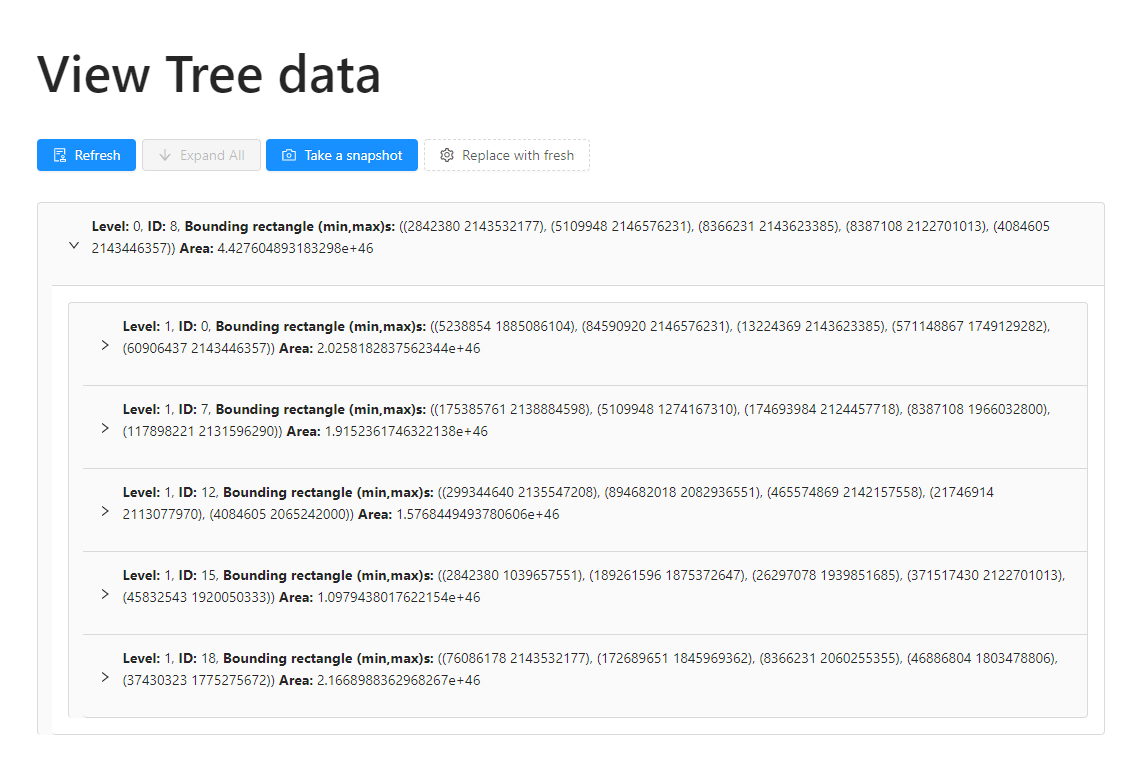
\includegraphics[width=\textwidth]{Data.png}
    \caption{Záložka Data}
    \label{fig:data}
\end{figure}

\begin{figure}
    \centering
    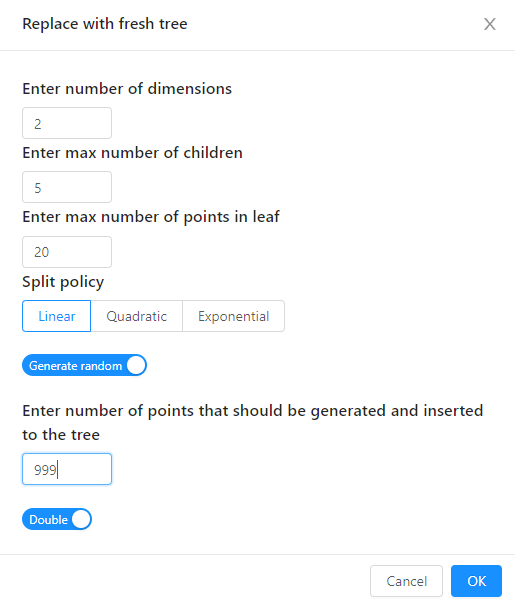
\includegraphics[width=.75\textwidth]{Replace.png}
    \caption{Záložka Data, formulář Replace with fresh}
    \label{fig:replace}
\end{figure}




\subsubsection*{Visualize}
Na záložce visualize je kanvas, který graficky zobrazuje body stromu a MBR uzlů, pokud je strom dimenze 2. Tato záložka zobrazuje, jak jsou body uloženy v uzlech a jak jsou postupně vytářeny další uzly a obdélníky. Na této vizualizaci lze pozorovat rozdíly mezi jednotlivými použitými metodami pro rozdělení plných uzlů. V příkladu na obrázku je použitý Quadratic split. Obrázek \ref{fig:visualize}.
\begin{figure}
    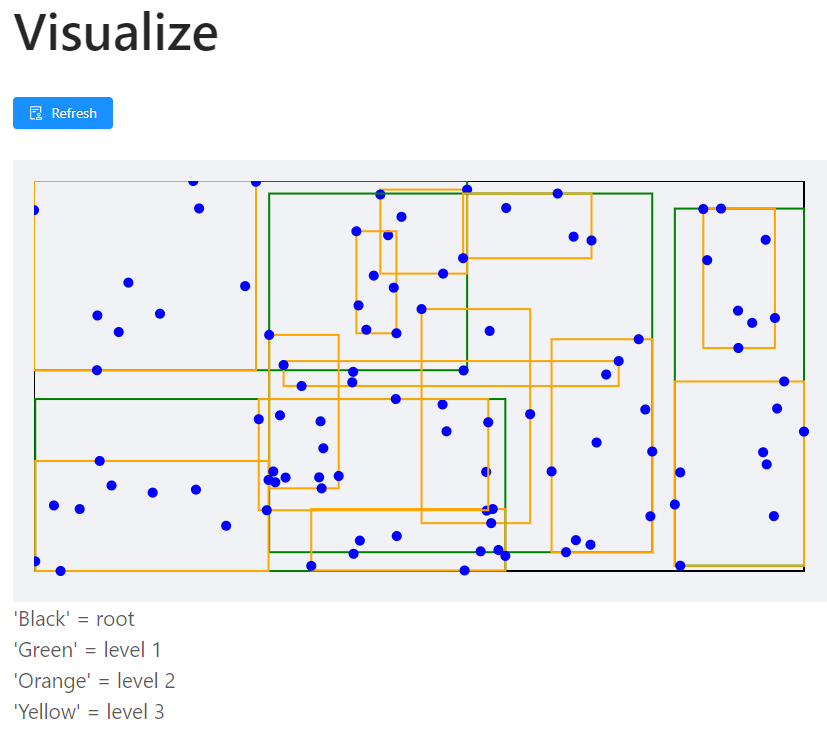
\includegraphics[width=\textwidth]{Visualize.png}
    \caption{Záložka Visualize}
    \label{fig:visualize}
\end{figure}

\subsubsection*{Snapshots}
Záložka Snapshots tvoří rozhraní pro práci s uloženými Snapshoty stromů. Snapshot stromu je možné načíst, smazat, nebo stáhnout v JSON formátu.\ref{fig:snapshot}
\begin{figure}
    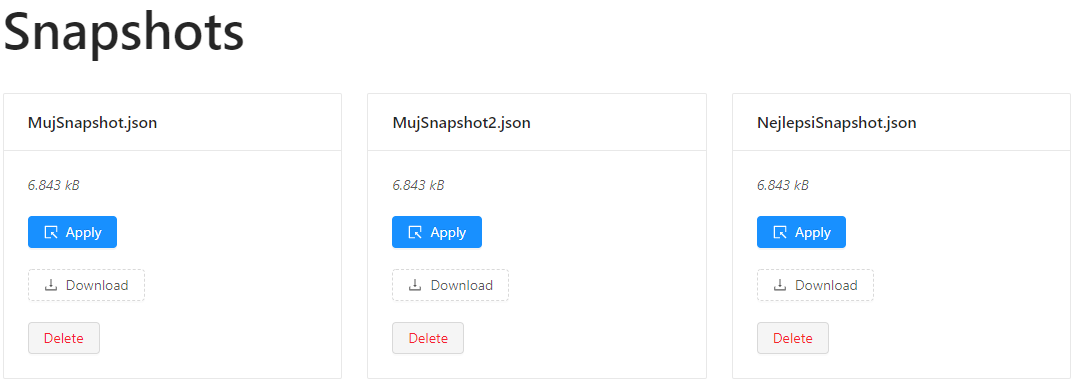
\includegraphics[width=\textwidth]{Snapshot.png}
    \caption{Záložka Snapshots}
    \label{fig:snapshot}
\end{figure}

\section{Experimentální sekce} \label{sec:exp}
Při vytváření R-stromu můžeme nastavit několik parametrů.

\begin{itemize}
	\item Number of dimensions
    \item Max number of children
    \item Max number of points in leaf
    \item Split policy
\end{itemize}

S těmito parametry je možné pohybovat a sledovat rychlost vytvoření stromu nebo rychlost dotazů nad stromem v závislosti na těchto parametrech. Dále můžeme porovnávat rychlost dotazů nad stromem s rychlostí dotazů provedených nad stejnými daty, ale lineárně.

\subsection{Rychlost vkládání bodů}

V tomto testu jsme vygenerovali 100 000 náhodných bodů, které jsme vložili do stromu a měřili rychlost této operace v závislosti na parametrech Max number of children a Max number of points in leaf, které jsou oba nastaveny na stejnou hodnotu, uvedenou na ose $x$. Parametr Number of dimensions byl nastaven na 3. Test jsme provedli desetkrát a výsledky zprůměrovali pro vyšší přesnost měření.

V grafu můžeme vidět, že zatímco Linear a Quadratic algoritmy se zvyšujícím se počtem Max children běží pořád téměř stejnou dobu, Exponential algoritmus se podle očekávání výrazně zpomaluje. Obrázek \ref{fig:insert}

\begin{figure}
    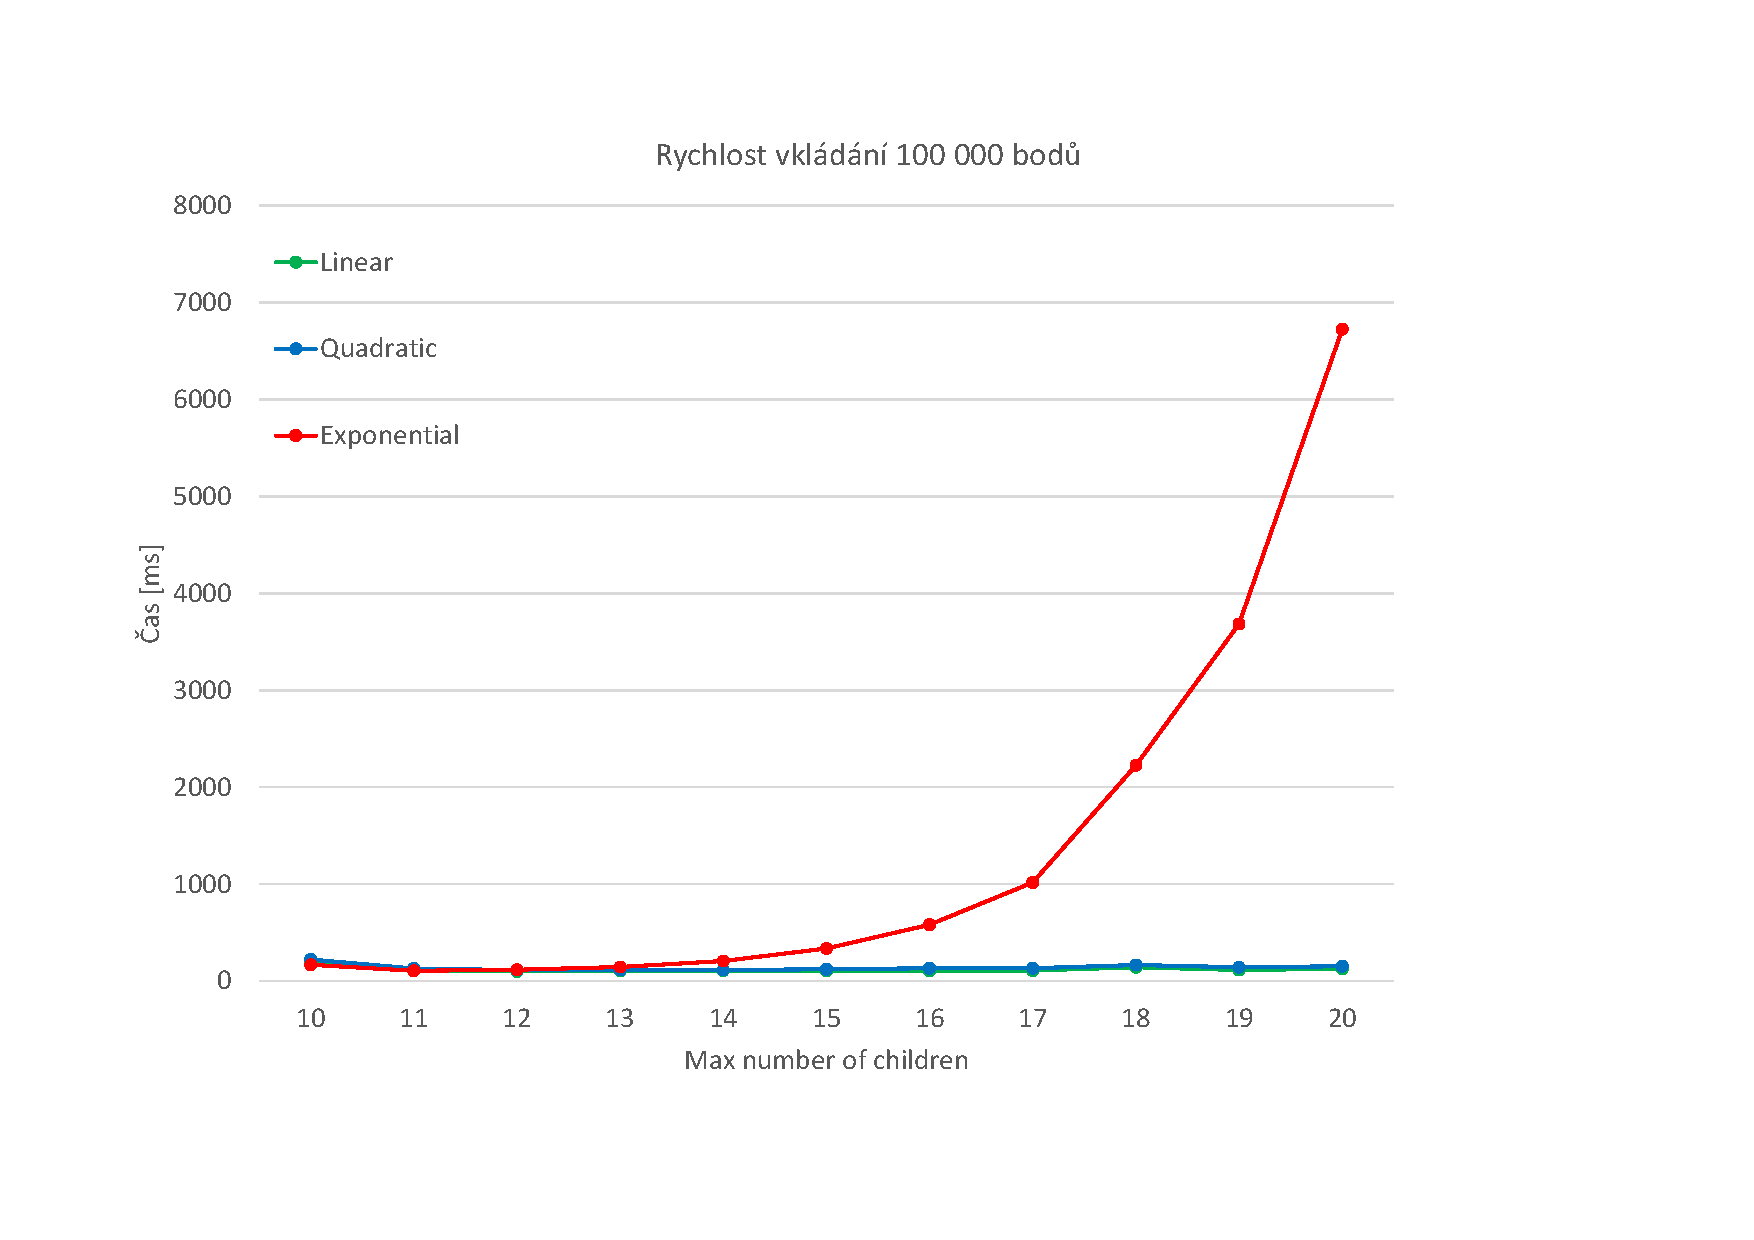
\includegraphics[width=\textwidth]{Insert.pdf}
    \caption{Graf rychlosti vkládání při použití různých Split policy}
    \label{fig:insert}
\end{figure}

\subsection{Rychlost dotazování}
V testu rychlosti dotazů jsme nastavili Number of dimensions na 2 a Max number of children na 15. Poté jsme náhodně vygenerovali 2 000 000 bodů, které byly vloženy do stromu. Na tomto stromě jsme provedli 1000 náhodných dotazů. Range query - vybrán náhodný bod a náhodná range, KNN query - vybrá náhodný bod a hledáme 100 nejbližších sousedů.

Každý dotaz byl proveden tisíckrát a časy byly sečteny pro každé spuštění. Měřili jsme čas vytvoření datové struktury, čas běhu rozsahového dotazu a čas běhu KNN dotazu.
\begin{description}
	\item[Lineární vyhledávání] - vytvoření datové struktury pro lineární vyhledávání je velice rychlé, naopak dotazy jsou v porovnání s R-stromem pomalé a to zejména KNN dotaz
    \item[R-strom - Linear split] - vytvoření stromu trvá déle, nicméně na rychlosti dotazů můžeme pozorovat výrazné zlepšení
    \item[R-strom - Quadratic split] - vytváření stromu trvá nejdéle, ale na druhou stranu strom dosahuje nejlepších výsledků při porovnání rychlosti dotazů
\end{description}

\begin{figure}
    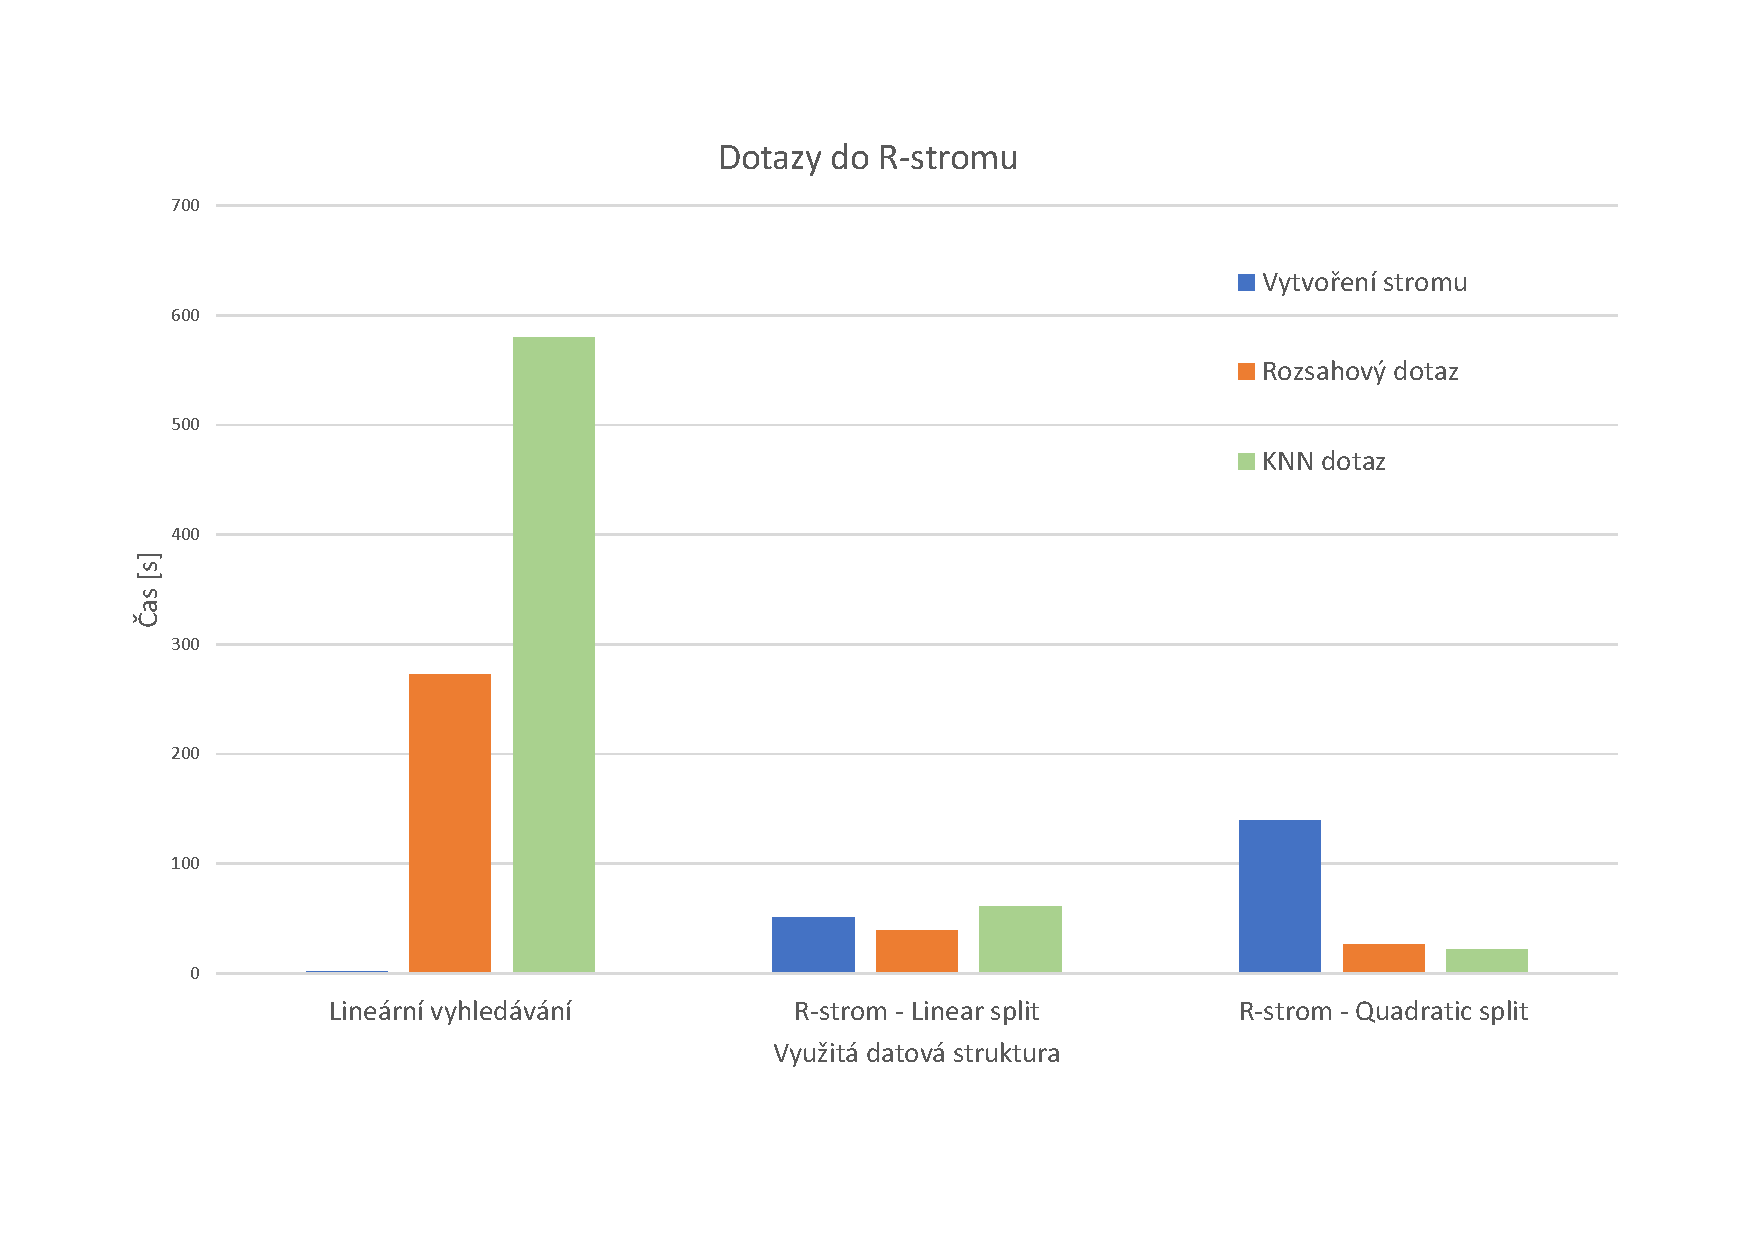
\includegraphics[width=\textwidth]{Query.pdf}
    \caption{Graf rychlosti vytvoření stromu a různých dotazů}
    \label{fig:query}
\end{figure}

\section{Diskuze}
Experimenty dopadly podle očekávání. Vkládání nových bodů do stromu s využitím exponenciálního algoritmu pro dělení uzlů se ukázalo jako velmi pomalé. Předpokládáme tedy, že největší využití bude mít algoritmus kvadratický. 

Linear split i Quadratic split algoritmy dosahují velmi dobrých výsledků v porovnání s lineárním vyhledáváním. Největší zlepšení je vidět při provádění KNN dotazů, které je u Quadratic splitu zhruba 3x rychlejší, než u Linear splitu a dokonce 25x rychlejší, než lineární vyhledávání.

Možná vylepšení - do R-stromu bychom mohli přidat i operaci mazání prvku. S touto operací souvisí i operace snížení počtu hladin stromu, když počet prvků v uzlu klesne pod určitou mez.

\section{Závěr}
Cílem bylo vytvořit R-strom, což se nám podařilo. Díky vytvořenému API je R-strom možné snadno použít pro nějaká reálná data. Mělo by tedy být relativně snadné použít tuto implementaci v některém reálném projektu, který pracuje s body v prostoru. Při rozsahových dotazech i KNN dotazech je strom několikanásobně rychlejší, než lineární vyhledávání a obecně strom i webová aplikace vracejí výsledky správně a rychle.

\clearpage
\bibliographystyle{csn690}
\begin{thebibliography}{1}

\bibitem{rtree}
\textit{MANOLOPOULOS, Yannis. R-trees: theory and applications.} London: Springer, c2006. Advanced information and knowledge processing. ISBN 18-523-3977-2.

\bibitem{nearest}
\textit{Nearest Neighbour Queries} [online]. [cit. 2019-05-07]. Dostupné z: \url{https://infolab.usc.edu/csci599/Fall2009/slides/Nearest\%20Neighbor\%20Queries\%20Slides.pdf}

\bibitem{newtonsoft}
\textit{Json.NET - Newtonsoft} [online]. [cit. 2019-05-07]. Dostupné z: \url{https://www.newtonsoft.com/json}

\bibitem{netstandard}
\textit{NETStandard.Library} [online]. [cit. 2019-05-07]. Dostupné z: \url{https://www.nuget.org/packages/NETStandard.Library/}

\bibitem{aspnetcore}
\textit{Microsoft.AspNetCore.All} [online]. [cit. 2019-05-07]. Dostupné z: \url{https://www.nuget.org/packages/Microsoft.AspNetCore.All/}


\bibitem{netcore}
\textit{Microsoft.NETCore.App} [online]. [cit. 2019-05-07]. Dostupné z: \url{https://www.nuget.org/packages/Microsoft.NETCore.App}

\bibitem{abstractions}
\textit{Microsoft.Extensions.PlatformAbstractions} [online]. [cit. 2019-05-07]. Dostupné z: \url{https://www.nuget.org/packages/Microsoft.Extensions.PlatformAbstractions/}

\bibitem{swagger}
\textit{Swashbuckle.AspNetCore} [online]. [cit. 2019-05-07]. Dostupné z: \url{https://www.nuget.org/packages/Swashbuckle.AspNetCore/5.0.0-rc2}

\bibitem{react}
\textit{React} [online]. [cit. 2019-05-07]. Dostupné z: \url{https://reactjs.org/}

\bibitem{ant}
\textit{Ant Design} [online]. [cit. 2019-05-07]. Dostupné z: \url{https://ant.design/}

\bibitem{konva}
\textit{Konva} [online]. [cit. 2019-05-07]. Dostupné z: \url{https://konvajs.org/}

\bibitem{dotnet}
\textit{Download .NET} [online]. [cit. 2019-05-08]. Dostupné z: \url{https://dotnet.microsoft.com/download}

\bibitem{nodejs}
\textit{Node.js} [online]. [cit. 2019-05-08]. Dostupné z: \url{https://nodejs.org/en/}

\bibitem{npm}
\textit{Node package manager} [online]. [cit. 2019-05-08]. Dostupné z: \url{https://www.npmjs.com/}


\end{thebibliography}



\end{document}
